\documentclass{article}
\usepackage{graphicx}
\usepackage[margin=1.5cm]{geometry}
\usepackage{amsmath}

\begin{document}

\title{Warm Up: Work and Energy}
\author{Prof. Jordan C. Hanson}

\maketitle

\section{Memory Bank}

\begin{itemize}
\item $v_f^2 = v_i^2 + 2 a \Delta x$ ... Kinematic equation without time.
\item $W = \vec{F} \cdot \Delta \vec{x}$ ... Definition of work
\item $\vec{F} = k\Delta \vec{x}$ ... Hooke's Law, or the force of a spring
\item $W = \frac{1}{2}k(\Delta x)^2$ ... Work done to compress or stretch a spring by $\Delta x$.
\item $KE = \frac{1}{2}m v^2$ ... Definition of Kinetic Energy
\item $W = KE_f - KE_i$ ... Work-energy theorem
\item $\int k x ~ dx = \frac{1}{2}x^2 + C$ ... The \textit{integral} of a linear function, $f(x) = kx$, where $C$ is some constant.
\end{itemize}

\section{Work and Energy}

\begin{enumerate}
\item In Fig. \ref{fig:work} below, we see a spring that is compressed by $\Delta \vec{x}$.  (a) If the spring ($k = 300$ N/m) is compressed a distance of 5 cm to launch a 250 mg object, what is the speed of the object as it leaves the spring?  (b) How high does the object rise, if it is shot straight upwards? \\ \vspace{2cm}
\begin{figure}
\centering
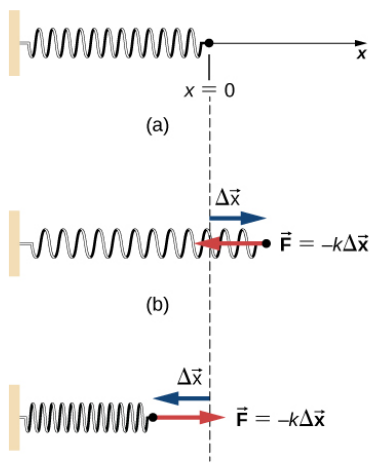
\includegraphics[width=0.2\textwidth]{springWork.png}
\caption{\label{fig:work} When a spring is compressed by a distance $\Delta x$, this requires a force $\vec{F} = k\Delta \vec{x}$ because the spring presses back with $\vec{F} = -k\Delta \vec{x}$.}
\end{figure}
\item Recall the kinematic equation without time (memory bank). (a) Rearrange the equation so that the velocity terms are on the left side, and divide both sides by 2.  (b) Multiply both sides by mass, $m$.  (c) Show that the right side is equal to the work done on $m$, and that we have proved a version of the work-energy theorem.
\end{enumerate}

\end{document}
